\documentclass[12pt,a4paper]{article}

\usepackage{fontspec}
\usepackage{polyglossia}
\setdefaultlanguage{russian}
\setotherlanguage{english}
\setmainfont{Times New Roman}[Ligatures=TeX]
\setmonofont{Menlo}[Scale=0.80]
\newfontfamily\cyrillicfont{Times New Roman}[Ligatures=TeX]
\newfontfamily\cyrillicfonttt{Menlo}[Scale=0.80]

\usepackage[left=2.2cm,right=1.5cm,top=2cm,bottom=2cm]{geometry}
\usepackage{graphicx}
\usepackage{float}
\usepackage{fvextra}
\usepackage{enumitem}
\usepackage{caption}
\usepackage{booktabs}
\usepackage[hidelinks]{hyperref}
\usepackage{xurl}

\linespread{1.08}
\setlength{\parindent}{1.25cm}
\setlist{nosep,leftmargin=*}
\widowpenalty=10000
\clubpenalty=10000
\graphicspath{{../screenshots/}}
\fvset{fontsize=\scriptsize,frame=single,framesep=1.5mm,breaklines=true,breakanywhere=true}
\captionsetup{font=small,labelsep=period}
\newcommand{\code}[1]{\texttt{#1}}
\sloppy
\setlength{\emergencystretch}{4em}
\newcommand{\NfPause}{17:00:29.749}
\newcommand{\NfWatch}{10,56}
\newcommand{\NfLead}{10,57}
\newcommand{\FPause}{17:01:39.247}
\newcommand{\FWatch}{11,06}
\newcommand{\FLead}{11,07}
\newcommand{\DNfPause}{17:04:08.966}
\newcommand{\DNfWatch}{10,19}
\newcommand{\DNfLead}{10,19}
\newcommand{\DFPause}{17:05:17.898}
\newcommand{\DFWatch}{11,26}
\newcommand{\DFLead}{11,26}
\newcommand{\EphGone}{29}
\newcommand{\EphReal}{33}


\begin{document}

\begin{titlepage}
\centering
\vspace*{3cm}
{\large Домашнее задание 4\par}
\vspace{1.5cm}
{\LARGE\bfseries Обеспечение отказоустойчивости\\ средствами Apache ZooKeeper\par}
\vspace{2cm}
\begin{flushright}
Выполнил: Апрелков Михаил Павлович\\
ИИИ-3-ИнжДан-1-5
\end{flushright}
\vfill
2026
\end{titlepage}
\setcounter{page}{2}

\section{Стенд}

MacBook (Apple M5 Pro, macOS 26). OpenJDK 17 (\code{JAVA\_HOME} в \code{infra/env.sh}), ZooKeeper 3.9.6 в трёх
копиях \code{zk/zk1..3} на одной машине, клиенты --- \code{zkCli.sh} и Python-библиотека kazoo. Координатор --- MapReduce из ДЗ-3
(пары навыков вакансий C/C++, данные в RustFS со стенда ДЗ-2). Репозиторий: \url{https://github.com/XTrapp1r/de-hw4-zookeeper},
вывод всех команд --- \code{logs/*.log}, журналы координаторов --- \code{logs/<прогон>/coord-A.log}, \code{coord-B.log}.

\begin{Verbatim}
$ echo "JAVA_HOME=$JAVA_HOME"; java -version
JAVA_HOME=/opt/homebrew/opt/openjdk@17/libexec/openjdk.jdk/Contents/Home
openjdk version "17.0.21.0.3" 2026-10-24
OpenJDK Runtime Environment Homebrew (build 17.0.21.0.3+0)
OpenJDK 64-Bit Server VM Homebrew (build 17.0.21.0.3+0, mixed mode, sharing)
$ zk/zk1/bin/zkServer.sh version 2>&1 | tail -1
Apache ZooKeeper, version 3.9.6 2026-09-03 19:29 UTC
\end{Verbatim}


\section{Ансамбль}

Строки \code{server.N} у всех трёх конфигураций одинаковые, свои только \code{clientPort}, порт AdminServer и \code{dataDir}.
В \code{dataDir} лежит \code{myid} с номером сервера.

\begin{Verbatim}
$ cat zk/zk1/conf/zoo.cfg
tickTime=2000
initLimit=10
syncLimit=5
minSessionTimeout=4000
maxSessionTimeout=40000
4lw.commands.whitelist=srvr,stat,ruok,mntr,conf,cons,dump
server.1=127.0.0.1:2888:3888
server.2=127.0.0.1:2889:3889
server.3=127.0.0.1:2890:3890

dataDir=data/zk1
clientPort=2181
admin.serverPort=8081
$ diff zk/zk1/conf/zoo.cfg zk/zk2/conf/zoo.cfg; diff zk/zk1/conf/zoo.cfg zk/zk3/conf/zoo.cfg; true
< dataDir=data/zk1
< clientPort=2181
< admin.serverPort=8081
> dataDir=data/zk2
> clientPort=2182
> admin.serverPort=8082
< dataDir=data/zk1
< clientPort=2181
< admin.serverPort=8081
> dataDir=data/zk3
> clientPort=2183
> admin.serverPort=8083
$ for i in 1 2 3; do echo "data/zk$i/myid = $(cat data/zk$i/myid)"; done
data/zk1/myid = 1
data/zk2/myid = 2
data/zk3/myid = 3
\end{Verbatim}


После \code{zkServer.sh start} один сервер --- лидер, два --- последователи:

\begin{Verbatim}
$ for i in 1 2 3; do zk/zk$i/bin/zkServer.sh status; done
Mode: follower
Mode: follower
Mode: leader
$ for i in 1 2 3; do echo "zk$i: $(curl -s localhost:808$i/commands/leader | tr -d "\n ")"; done
zk1: {"is_leader":false,"leader_id":3,"leader_ip":"127.0.0.1","command":"leader","error":null}
zk2: {"is_leader":false,"leader_id":3,"leader_ip":"127.0.0.1","command":"leader","error":null}
zk3: {"is_leader":true,"leader_id":3,"leader_ip":"127.0.0.1","command":"leader","error":null}
\end{Verbatim}


\begin{figure}[H]
\centering
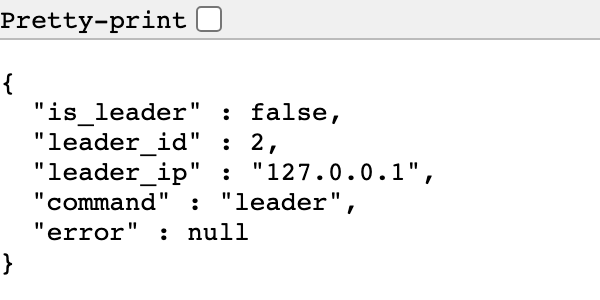
\includegraphics[width=0.32\textwidth]{admin_zk1.png}\hfill
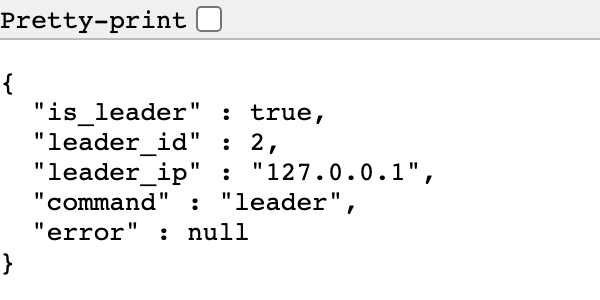
\includegraphics[width=0.32\textwidth]{admin_zk2.png}\hfill
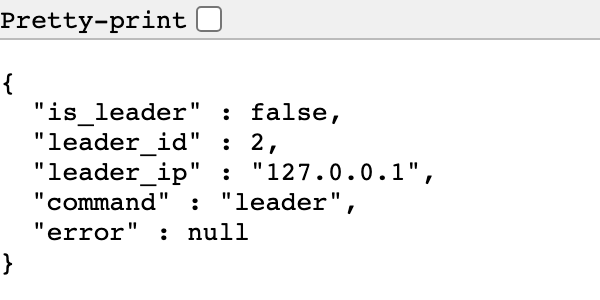
\includegraphics[width=0.32\textwidth]{admin_zk3.png}
\caption{AdminServer \code{/commands/leader} трёх серверов}
\end{figure}

Останавливаем лидера: оставшиеся два выбирают нового, запись и чтение работают. Останавливаем второй сервер: последний жив
(\code{imok}), но без кворума не обслуживает клиентов, сессия не открывается. После запуска обоих кворум и данные на месте.

\begin{Verbatim}
$ zk/zk3/bin/zkServer.sh stop
Stopping zookeeper ... STOPPED
$ zkstatus
zk1 (порт 2181): Mode: follower
zk2 (порт 2182): Mode: leader
zk3 (порт 2183): Error contacting service. It is probably not running.
$ zkcli 127.0.0.1:2181 set /hw4-check 'изменено через zk1, когда работают 2 из 3'; zkcli 127.0.0.1:2182 get -s /hw4-check | grep -E 'изменено|dataVersion'
изменено через zk1, когда работают 2 из 3
dataVersion = 1
$ python src/zkctl.py probe
кворум есть: сессия 0x200012d9ac10001 на 127.0.0.1:2182, setData /hw4-probe=2026-11-14T16:59:06 -> version 9, прочитано 2026-11-14T16:59:06
$ zk/zk2/bin/zkServer.sh stop
Stopping zookeeper ... STOPPED
$ zkstatus
zk1 (порт 2181): Error contacting service. It is probably not running.
zk2 (порт 2182): Error contacting service. It is probably not running.
zk3 (порт 2183): Error contacting service. It is probably not running.
$ echo ruok | nc localhost 2181; echo; echo srvr | nc localhost 2181
imok
This ZooKeeper instance is not currently serving requests
$ python src/zkctl.py probe
НЕТ КВОРУМА: за 5.1 с не удалось открыть сессию (KazooTimeoutError); попыток соединения, оборванных серверами: 15 - ансамбль не обслуживает клиентов
[exit code 1]
$ with_timeout 20 zk/zk1/bin/zkCli.sh -server 127.0.0.1:2181 get /hw4-check 2>&1 | grep -v -E '^(WATCHER::|$)' | tail -4
KeeperErrorCode = ConnectionLoss for /hw4-check
$ zk/zk3/bin/zkServer.sh start; zk/zk2/bin/zkServer.sh start
Starting zookeeper ... STARTED
Starting zookeeper ... STARTED
$ zkstatus
zk1 (порт 2181): Mode: leader
zk2 (порт 2182): Mode: follower
zk3 (порт 2183): Mode: follower
$ zkcli 127.0.0.1:2181,127.0.0.1:2182,127.0.0.1:2183 get -s /hw4-check | grep -E 'изменено|dataVersion'
изменено через zk1, когда работают 2 из 3
dataVersion = 1
\end{Verbatim}


\textbf{Эфемерный узел.} Во втором окне \code{zkCli} создаёт узел \code{-e}, в первом виден его \code{ephemeralOwner}. Окно
закрыто без \code{quit} --- узел исчез через \EphGone~с: истёк тайм-аут сессии \code{zkCli} 30~с, который сервер отсчитывает
от последнего пакета клиента. При \code{quit} узел исчезает сразу.

\begin{Verbatim}
$ grep -v -E '^(WATCHER::|WatchedEvent|Connecting|Welcome|JLine|$)' logs/02_window2.log | sed 's/\[zk: /\n[zk: /g' | grep -v '^$'
[zk: 127.0.0.1:2182(CONNECTED) 0] Created /hw4-ephemeral
ephemeralOwner = 0x200012de6da0001
$ for p in 2181 2182 2183; do echo dump | nc localhost $p | grep -A3 "Sessions with Ephemerals"; done
Sessions with Ephemerals (1):
0x200012de6da0001:
    /hw4-ephemeral
16:59:35.187 закрываю окно 2
...
17:00:00.110 через 25 с: /hw4-ephemeral ещё есть (сессия окна 2 ещё не истекла)
17:00:04.782 узел /hw4-ephemeral исчез через 29 с после закрытия окна (сессия zkCli 30 с истекла)
$ zkcli 127.0.0.1:2181 get -s /hw4-ephemeral2 | grep -E 'второй|ephemeralOwner'
второй эфемерный
ephemeralOwner = 0x300012de3710002
$ zkcli 127.0.0.1:2181 stat /hw4-ephemeral2
Node does not exist: /hw4-ephemeral2
\end{Verbatim}


То же в настоящей второй вкладке терминала, закрытой крестиком (\code{logs/02\_window2\_terminal.log}):

\begin{Verbatim}
[zk: 127.0.0.1:2182(CONNECTED) 0] Created /hw4-window2
ephemeralOwner = 0x200011d545e0000
16:42:33.169 окно 2 закрыто
16:43:06.200 узел /hw4-window2 исчез через 33 с
\end{Verbatim}


\section{Координатор}

\code{src/coordinator.py} --- мастер MapReduce из ДЗ-3 (логика расчёта не менялась) поверх ZooKeeper:
\begin{itemize}
\item выбор лидера --- эфемерные последовательные узлы \code{/hw4/skills/election/c\_N}, запасной ставит watch на узел предшественника;
\item эпоха --- версия узла \code{/hw4/skills/epoch}, новый лидер увеличивает её через \code{setData};
\item чекпоинт --- узел \code{/hw4/skills/checkpoint/map-NNNN} на каждую готовую задачу, новый лидер пропускает отмеченные;
\item результат --- CSV в S3 и указатель \code{/hw4/skills/result}. При \code{FENCING=1} указатель пишется транзакцией
\code{check(epoch, version=моя\_эпоха) + setData}.
\end{itemize}

Без отказов расчёт идёт около секунды, поэтому в сценариях каждая из 46 map-задач дополнительно спит 1~с (\code{--slow 1.0}).
Контрольный прогон без задержки совпадает с ДЗ-3:

\begin{Verbatim}
$ RUN=03_single COORD_ID=A python src/coordinator.py --slow 0 | grep -v -E 'map-[0-9]+ attempt|kazoo: Connecting'
17:00:17.715 [A] КОНТРОЛЬ: вакансий варианта 1815, навыков 57 (сумма 8078), пар 1227 (сумма 17072), троек 6630 (сумма 22826); sha256 pairs_k2.csv 955bdeaa2d72a9a6
$ python src/zkctl.py compare 03_single
ИТОГ: все результаты прогона побайтно совпали с ДЗ-3
\end{Verbatim}


Обе копии работают с тайм-аутом сессии 10~с --- это видно в журнале kazoo и в \code{cons} на сервере:

\begin{Verbatim}
$ grep -h 'Session created' logs/03_nofencing/coord-A.log logs/03_nofencing/coord-B.log
17:00:21.502 [A] kazoo: Session created, session_id: 72058890639376396 negotiated session timeout: 10000 connect timeout: 3333.3333333333335 read timeout: 6666.666666666667
17:00:21.716 [B] kazoo: Session created, session_id: 216174078714773510 negotiated session timeout: 10000 connect timeout: 3333.3333333333335 read timeout: 6666.666666666667
$ zkcons
сервер :2181  sid=0x100012de378000c    to=10000
сервер :2183  sid=0x300012de3710006    to=10000
\end{Verbatim}


\section{Пауза лидера без защиты}

Запускаются копии A и B, A становится лидером. Когда готовы 14 задач из 46, A получает \code{kill -STOP}, через 40~с ---
\code{kill -CONT}. Через \NfLead~с после паузы B стал лидером, пропустил 14 задач из чекпоинта, досчитал и записал результат.
Возобновлённый A не знает, что его сместили, и записывает результат второй раз: указатель версии 2 смотрит на результат
устаревшей эпохи~1. Контрольные числа обоих совпали с ДЗ-3.

\begin{figure}[H]
\centering
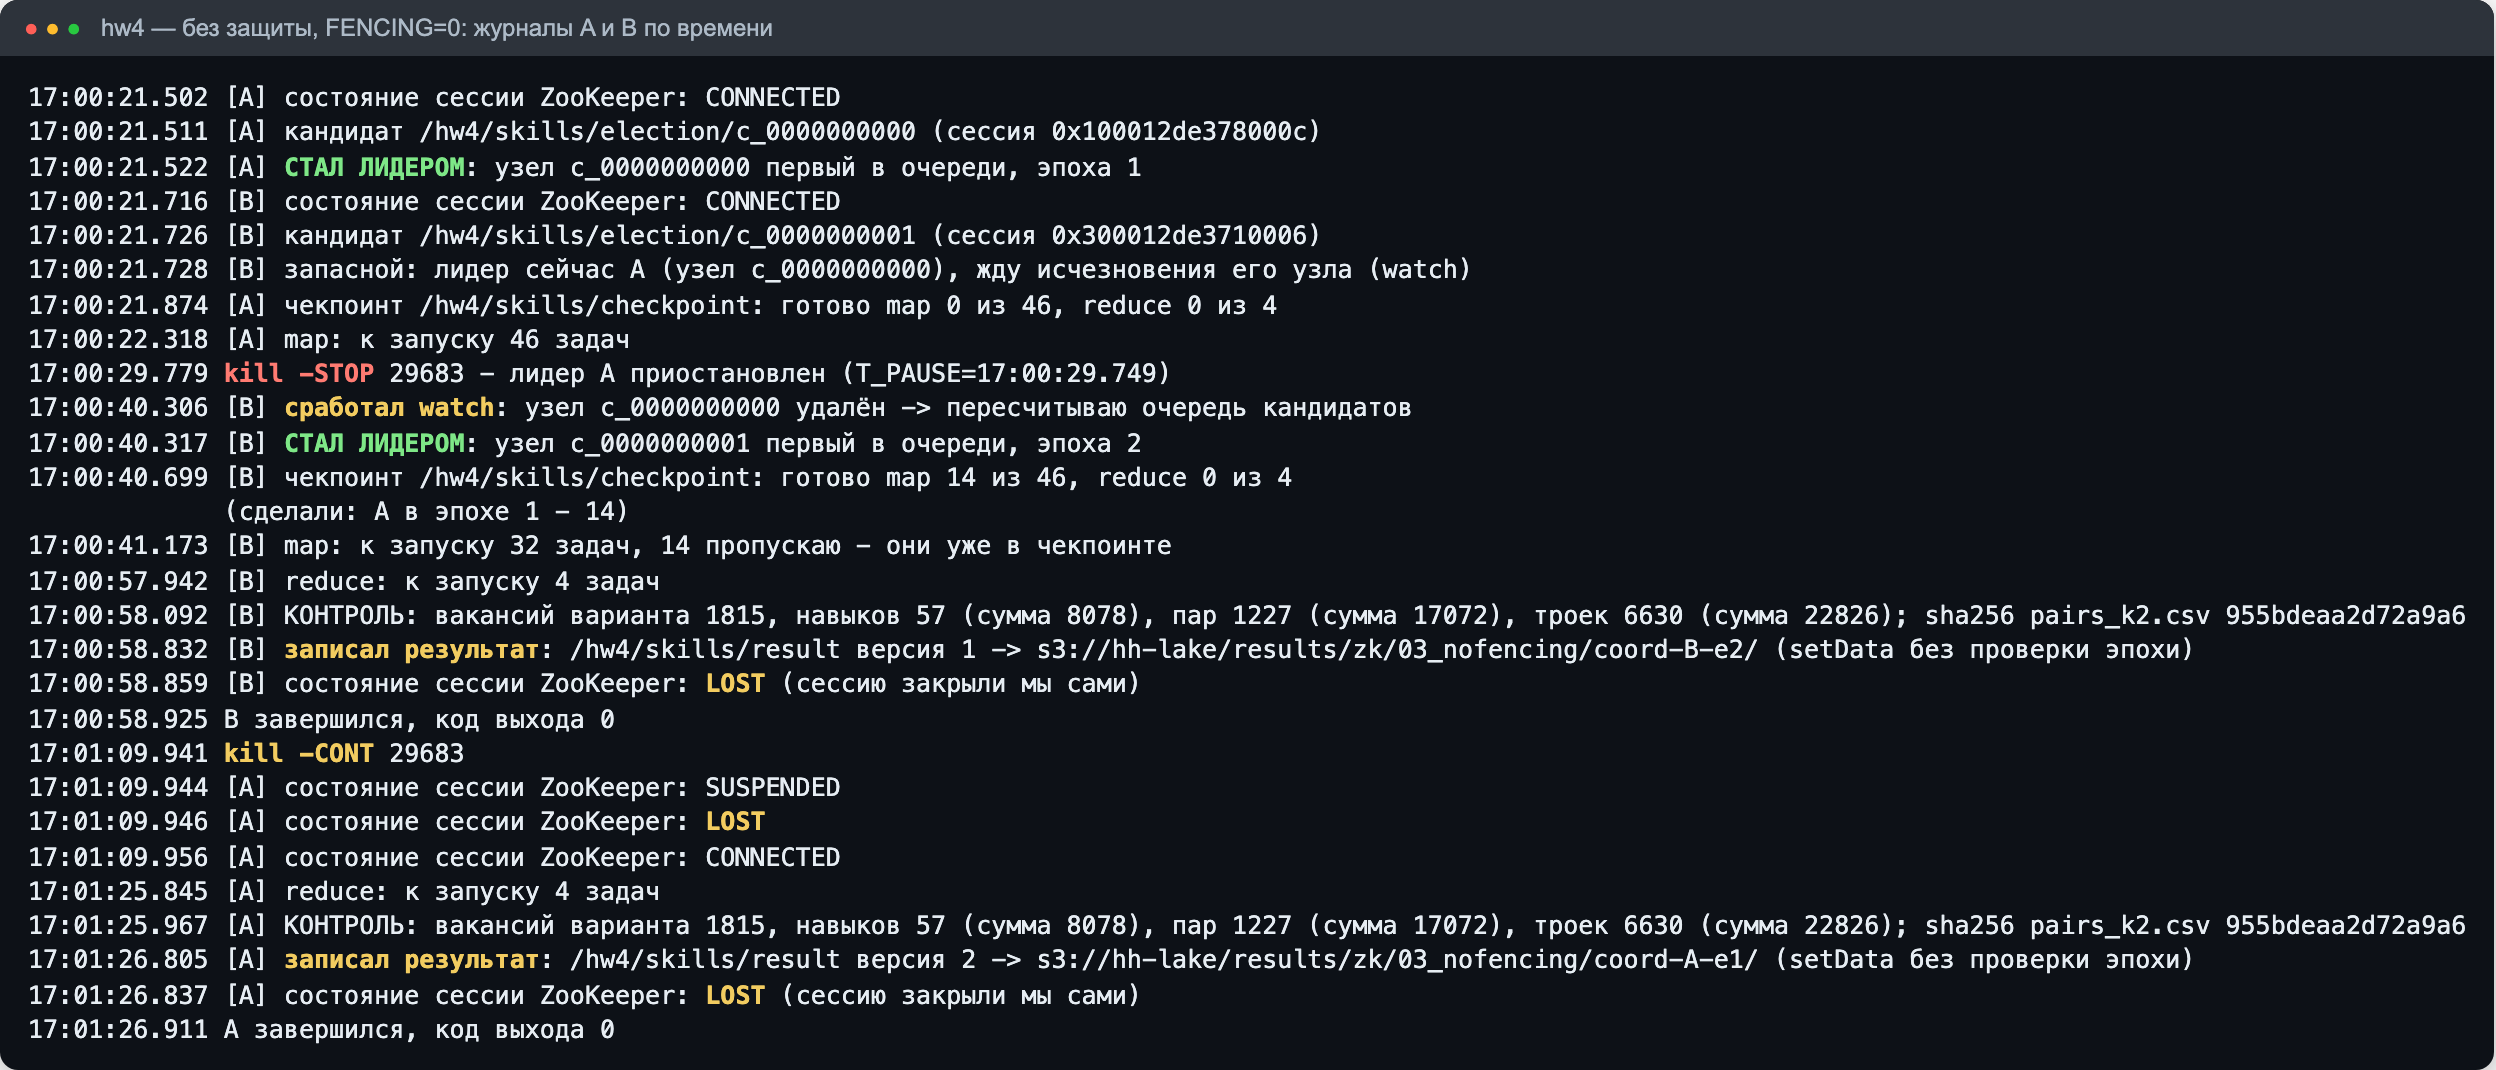
\includegraphics[width=\textwidth]{t_03_nofencing_timeline.png}
\caption{Журналы A и B по времени (\code{logs/03\_nofencing})}
\end{figure}

\begin{Verbatim}
$ grep -h -E 'записал результат|ОТКЛОНЕНА|BadVersion' logs/03_nofencing/coord-*.log | sort
17:00:58.832 [B] записал результат: /hw4/skills/result версия 1 -> s3://hh-lake/results/zk/03_nofencing/coord-B-e2/ (setData без проверки эпохи)
17:01:26.805 [A] записал результат: /hw4/skills/result версия 2 -> s3://hh-lake/results/zk/03_nofencing/coord-A-e1/ (setData без проверки эпохи)
$ zkcli 127.0.0.1:2181 get -s /hw4/skills/result | grep -E '^\{|dataVersion|mtime|mzxid'
{"by": "coord-A", "epoch": 1, "result": "s3://hh-lake/results/zk/03_nofencing/coord-A-e1/", "control": "вакансий варианта 1815, навыков 57 (сумма 8078), пар 1227 (сумма 17072), троек 6630 (сумма 22826)", "at": "2026-11-14T17:01:26.778"}
dataVersion = 2
$ python src/zkctl.py compare 03_nofencing
results/zk/03_nofencing/coord-A-e1/: вакансий 1815; skills_k1.csv: 57/8078/10d2050c1be05ce8; pairs_k2.csv: 1227/17072/955bdeaa2d72a9a6; triples_k3.csv: 6630/22826/336e66fb1832619c -> СОВПАДАЕТ с ДЗ-3  <- на него указывает /hw4/skills/result
results/zk/03_nofencing/coord-B-e2/: вакансий 1815; skills_k1.csv: 57/8078/10d2050c1be05ce8; pairs_k2.csv: 1227/17072/955bdeaa2d72a9a6; triples_k3.csv: 6630/22826/336e66fb1832619c -> СОВПАДАЕТ с ДЗ-3
ИТОГ: все результаты прогона побайтно совпали с ДЗ-3
\end{Verbatim}


\section{Пауза лидера с защитой по эпохе}

Тот же сценарий с \code{FENCING=1}. B стал лидером через \FLead~с и записал указатель. Запись A отклонена с
\code{BadVersionError}: эпоха уже 2, а A проверял версию 1. Указатель остался один --- от B.

\begin{figure}[H]
\centering
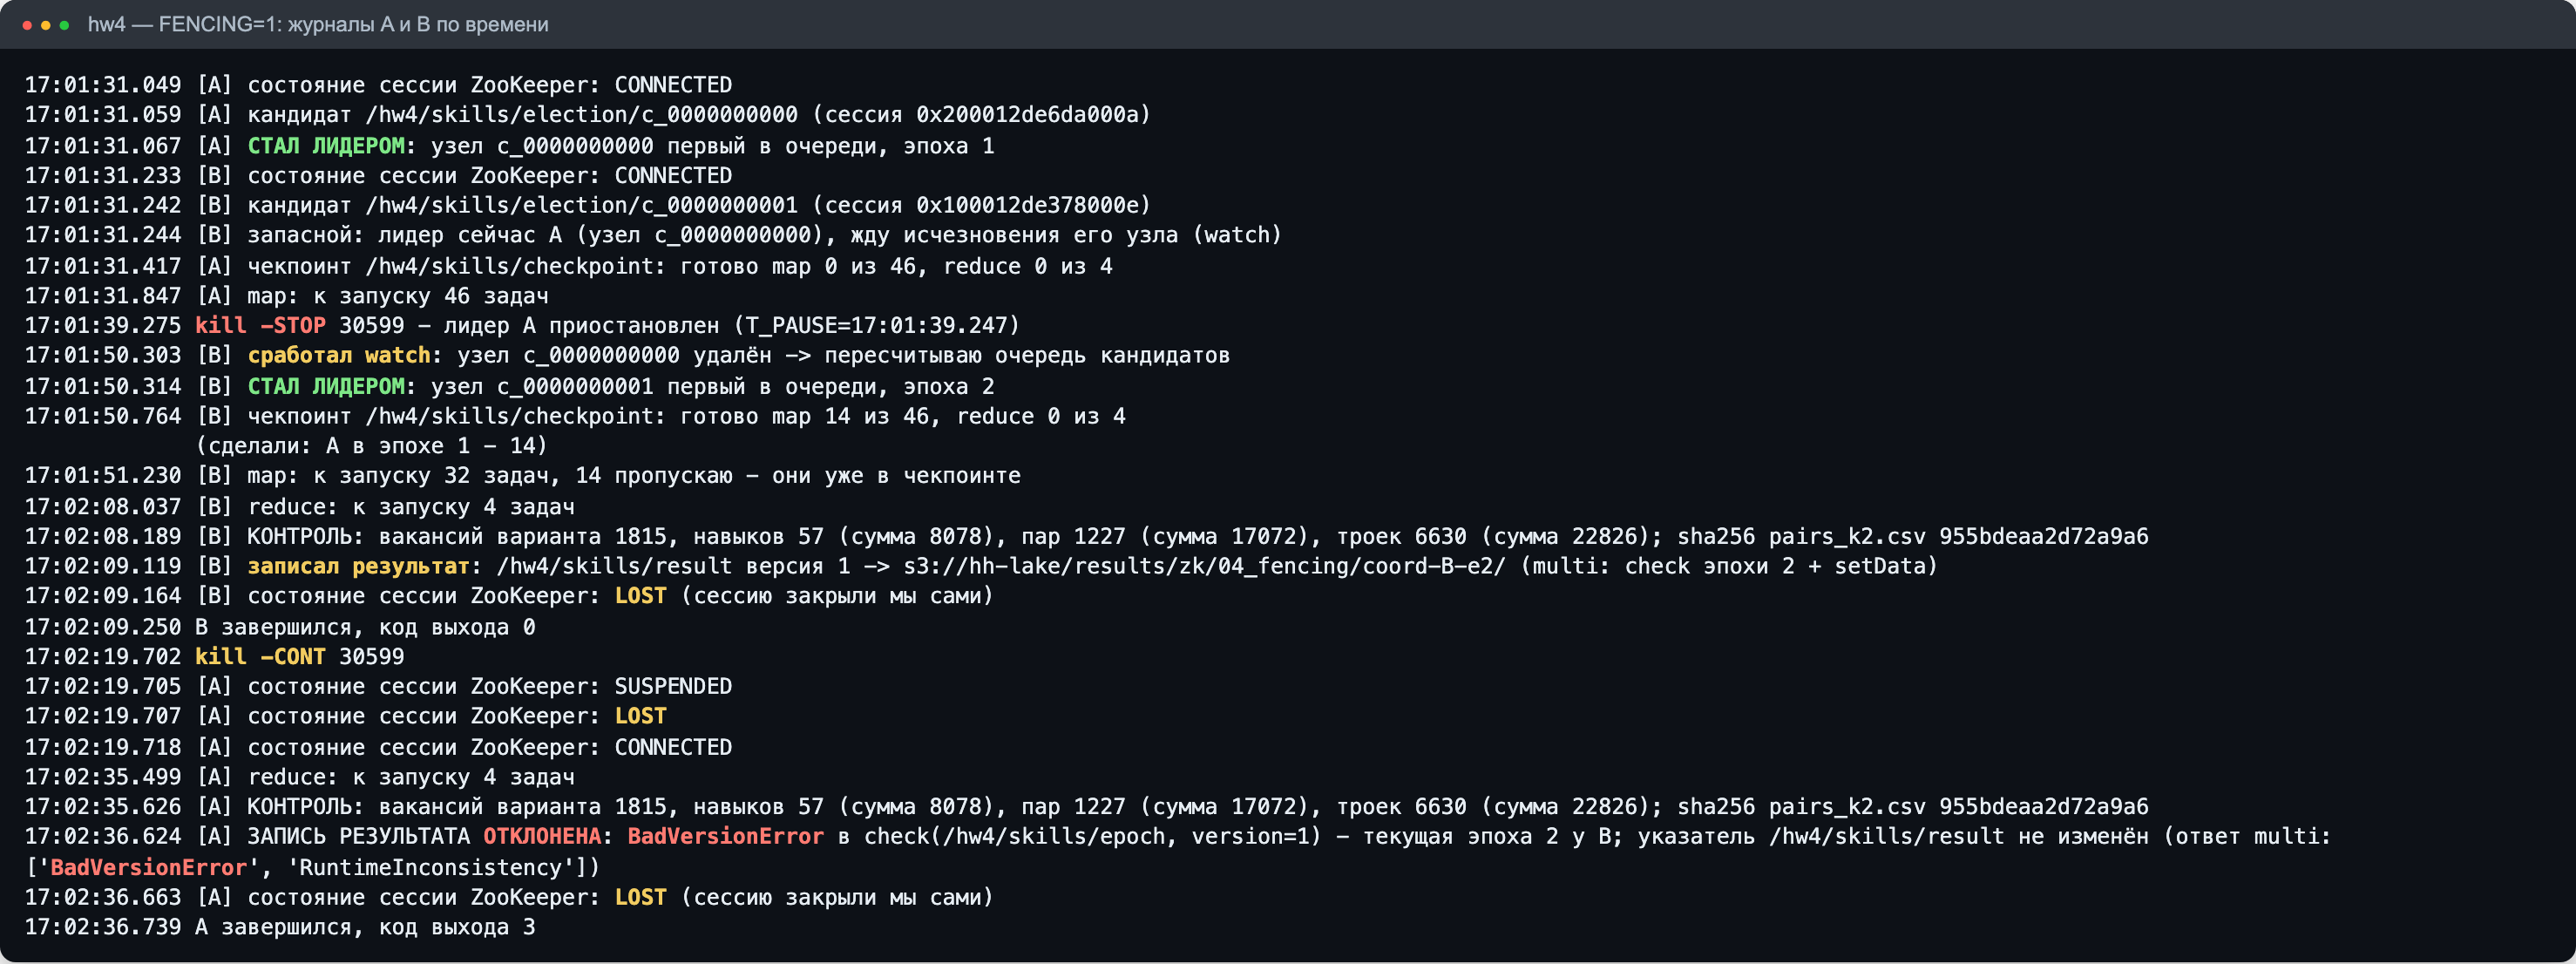
\includegraphics[width=\textwidth]{t_04_fencing_timeline.png}
\caption{Журналы A и B по времени (\code{logs/04\_fencing})}
\end{figure}

\begin{Verbatim}
$ grep -h -E 'записал результат|ОТКЛОНЕНА|BadVersion' logs/04_fencing/coord-*.log | sort
17:02:09.119 [B] записал результат: /hw4/skills/result версия 1 -> s3://hh-lake/results/zk/04_fencing/coord-B-e2/ (multi: check эпохи 2 + setData)
17:02:36.624 [A] ЗАПИСЬ РЕЗУЛЬТАТА ОТКЛОНЕНА: BadVersionError в check(/hw4/skills/epoch, version=1) - текущая эпоха 2 у B; указатель /hw4/skills/result не изменён (ответ multi: ['BadVersionError', 'RuntimeInconsistency'])
$ zkcli 127.0.0.1:2181 get -s /hw4/skills/result | grep -E '^\{|dataVersion|mtime|mzxid'
{"by": "coord-B", "epoch": 2, "result": "s3://hh-lake/results/zk/04_fencing/coord-B-e2/", "control": "вакансий варианта 1815, навыков 57 (сумма 8078), пар 1227 (сумма 17072), троек 6630 (сумма 22826)", "at": "2026-11-14T17:02:09.097"}
dataVersion = 1
$ python src/zkctl.py compare 04_fencing
results/zk/04_fencing/coord-A-e1/: вакансий 1815; skills_k1.csv: 57/8078/10d2050c1be05ce8; pairs_k2.csv: 1227/17072/955bdeaa2d72a9a6; triples_k3.csv: 6630/22826/336e66fb1832619c -> СОВПАДАЕТ с ДЗ-3
results/zk/04_fencing/coord-B-e2/: вакансий 1815; skills_k1.csv: 57/8078/10d2050c1be05ce8; pairs_k2.csv: 1227/17072/955bdeaa2d72a9a6; triples_k3.csv: 6630/22826/336e66fb1832619c -> СОВПАДАЕТ с ДЗ-3  <- на него указывает /hw4/skills/result
ИТОГ: все результаты прогона побайтно совпали с ДЗ-3
\end{Verbatim}


\section{Время смены лидера}

От \code{kill -STOP} лидера до строки <<СТАЛ ЛИДЕРОМ>> у запасного:

\begin{center}
\begin{tabular}{lccc}
\toprule
Прогон & Пауза & до watch, с & до нового лидера, с \\
\midrule
Без защиты & \NfPause & \NfWatch & \NfLead \\
FENCING=1 & \FPause & \FWatch & \FLead \\
Docker, без защиты & \DNfPause & \DNfWatch & \DNfLead \\
Docker, FENCING=1 & \DFPause & \DFWatch & \DFLead \\
\bottomrule
\end{tabular}
\end{center}

Почти всё время --- ожидание тайм-аута сессии 10~с с последнего пинга, плюс до одного такта (2~с), с которым сервер проверяет
истёкшие сессии. От watch до нового лидера --- около 10~мс.

\section{Вариант в Docker}

\code{compose.yaml} поднимает те же три сервера из образа \code{zookeeper:3.9.6-jre-17} на тех же портах.
\code{scripts/05\_docker.sh} повторяет все проверки: роли, потеря одного и двух серверов, эфемерный узел и оба сценария координатора.
Результат тот же (\code{logs/05\_docker*}).

\begin{Verbatim}
$ docker run --rm --entrypoint java zookeeper:3.9.6-jre-17 -version
openjdk version "17.0.21" 2026-10-20
$ for i in 1 2 3; do echo "--- docker exec zoo$i zkServer.sh status"; docker exec zoo$i zkServer.sh status 2>&1; done
--- docker exec zoo1 zkServer.sh status
Mode: follower
--- docker exec zoo2 zkServer.sh status
Mode: follower
--- docker exec zoo3 zkServer.sh status
Mode: leader
\end{Verbatim}


\begin{figure}[H]
\centering
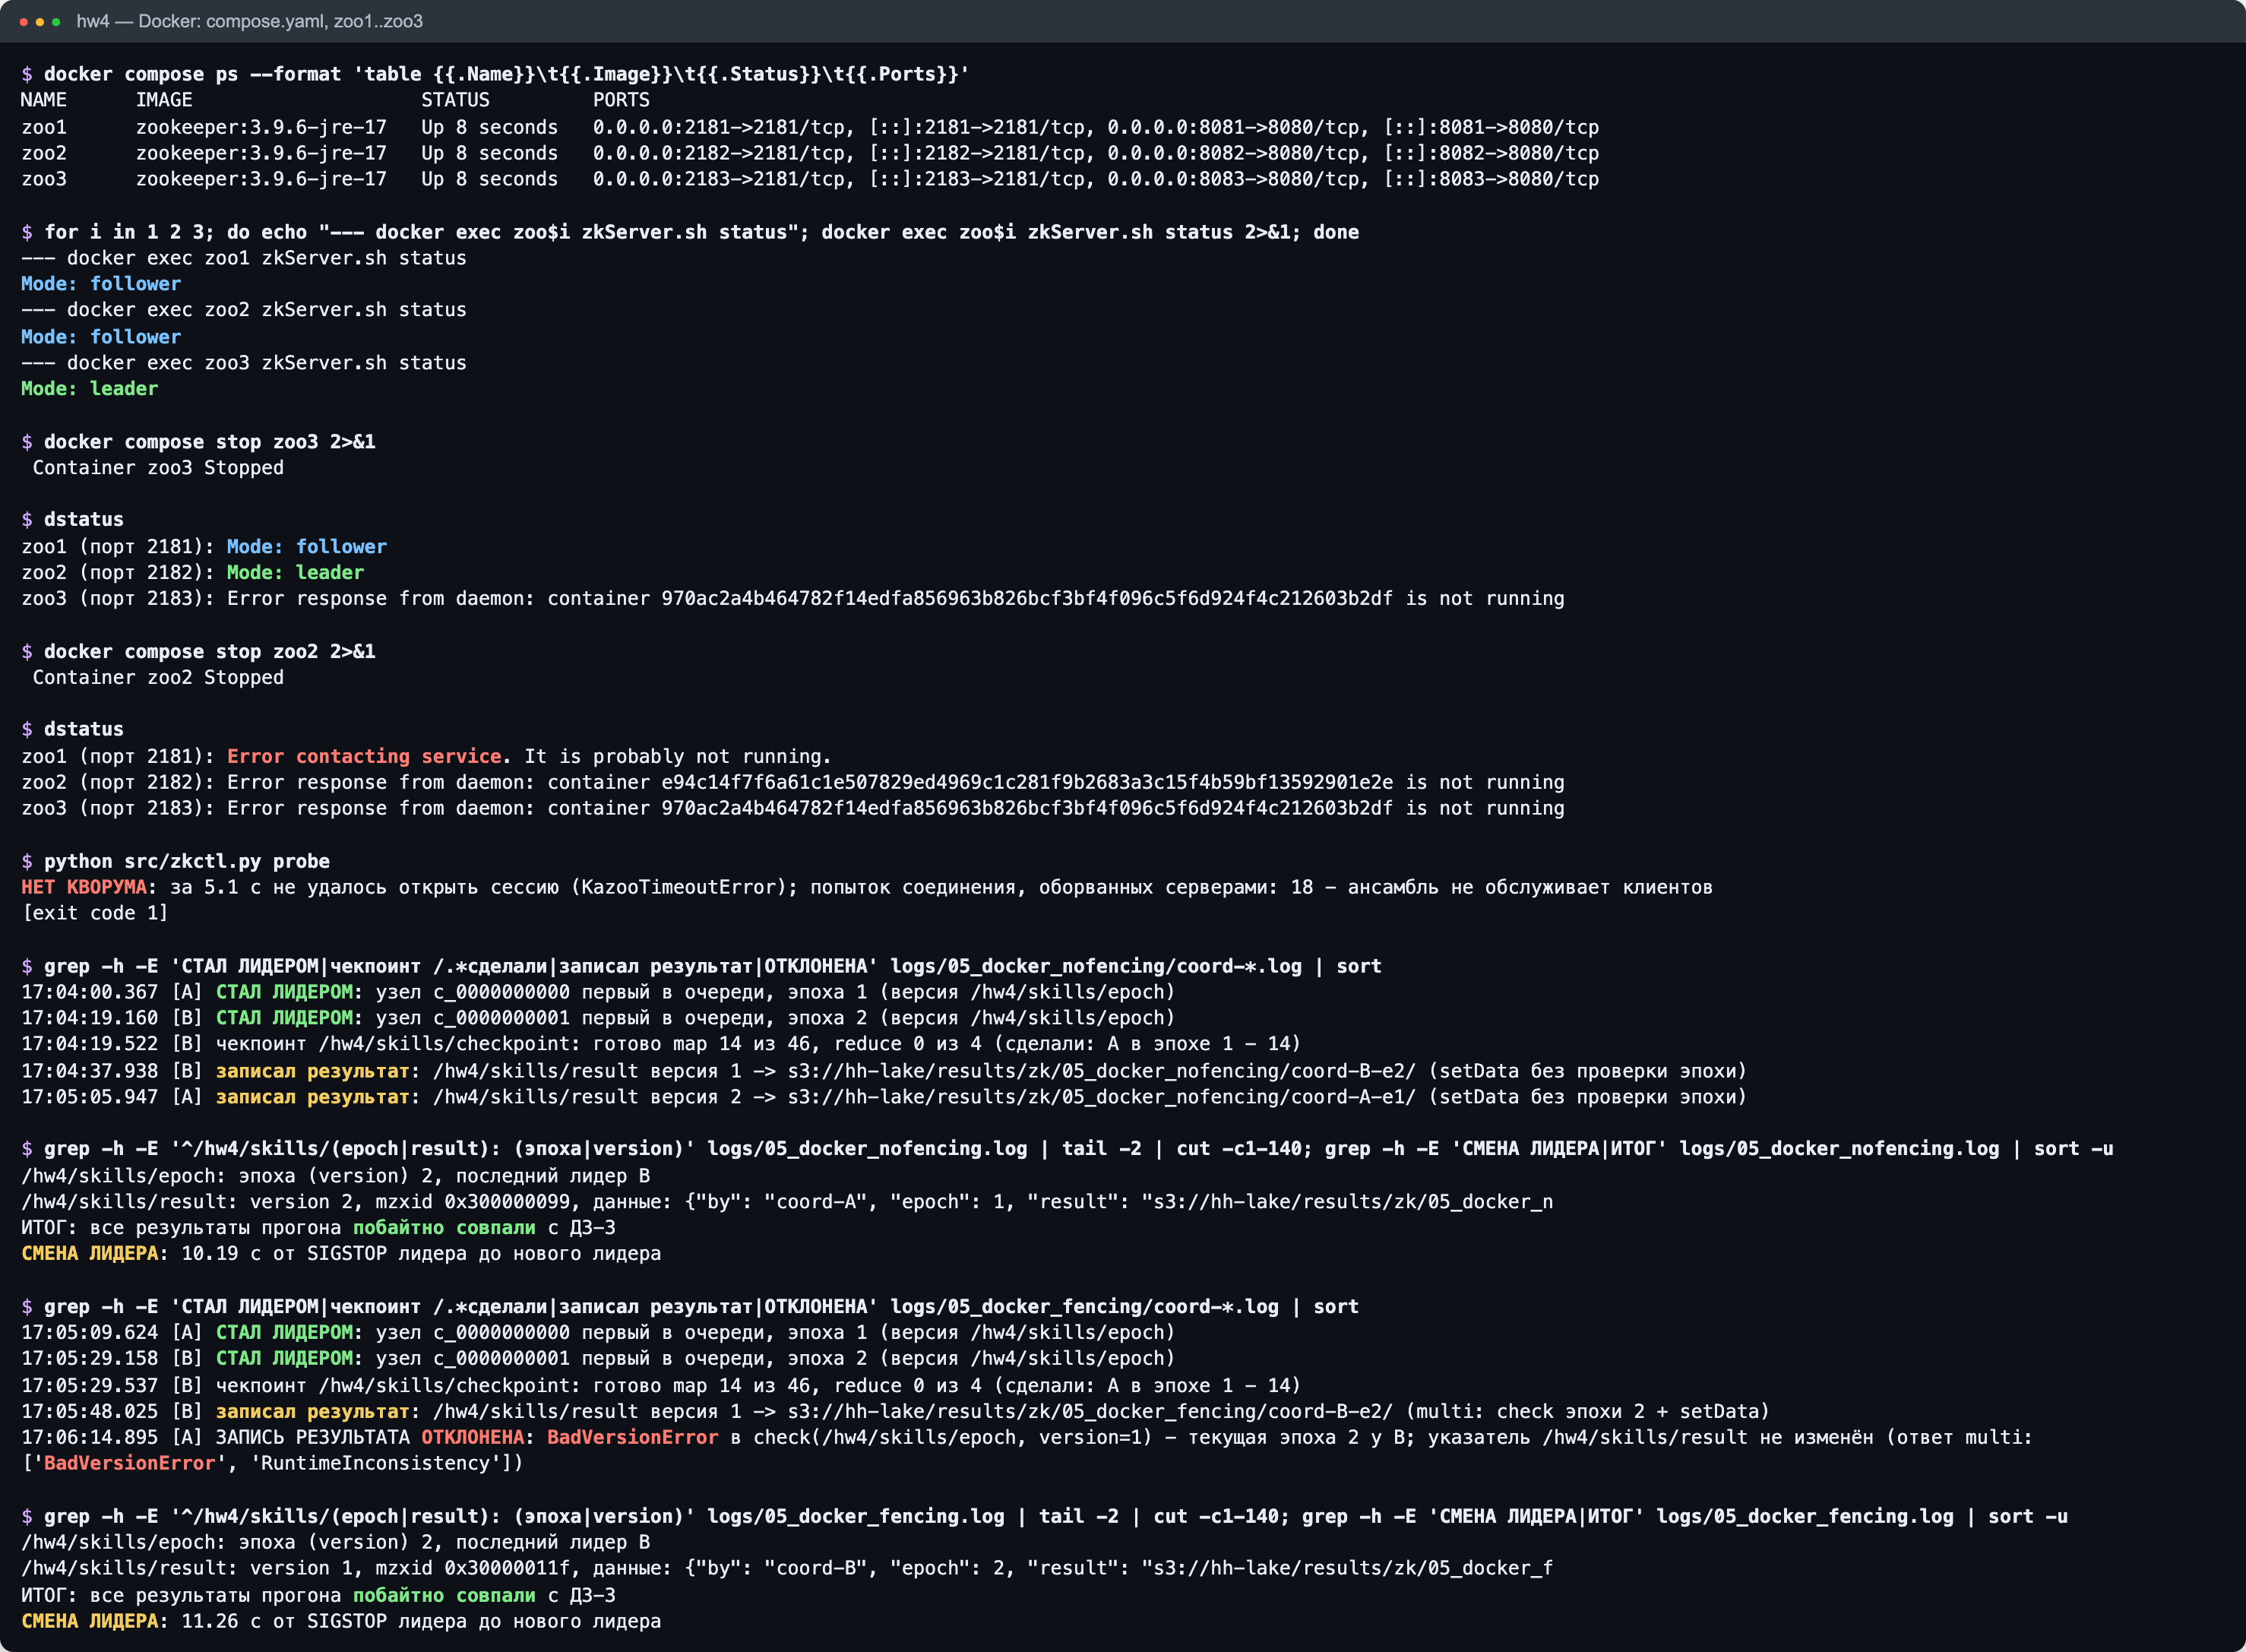
\includegraphics[width=\textwidth]{t4_docker.png}
\caption{Docker: роли, потеря серверов, итоги обоих сценариев}
\end{figure}

\section{Ответы на вопросы}

\subsection*{Почему серверов три, а не два и не четыре}

ZooKeeper пишет данные и выбирает лидера только с согласия большинства. Тогда две отрезанные друг от друга части не смогут
работать одновременно и разойтись. Из двух серверов большинство --- оба, и отказ любого останавливает сервис: это хуже, чем один
сервер. Из трёх большинство --- два, и ансамбль переживает отказ одного (это и видно в разделе~2). Из четырёх большинство --- три,
то есть отказ тоже переживается только один, а запись ждёт подтверждения от трёх серверов вместо двух. Поэтому размер ансамбля
берут нечётным: $2f+1$ серверов переживают $f$ отказов.

\subsection*{Почему защиту по эпохе проверяет получатель записи, а не ZooKeeper}

ZooKeeper только выбирает лидера и не участвует в самой записи результата. Со старым лидером он может лишь закрыть его сессию
и удалить его узел, но не может остановить процесс или отменить запись, которую тот уже отправил. Приостановленный A узнал о
потере сессии только после \code{kill -CONT}, через 30~с после того, как лидером стал B. Проверка <<я ещё лидер?>> перед записью
тоже не спасает: пауза может случиться между проверкой и записью. Надёжно отсечь старую запись может только тот, кто её
принимает, --- он сравнивает эпоху в той же операции, что и запись. У меня получатель --- узел-указатель: условие \code{check}
стоит в той же транзакции, что и \code{setData}. Для S3 или базы это был бы условный \code{PUT} или
\code{UPDATE ... WHERE epoch <= :e}.

\end{document}
